\documentclass[a4paper]{article}

% Global layout
\usepackage{fancyhdr, graphicx, hyperref, indentfirst, lastpage, setspace}
\usepackage[margin=40mm]{geometry}

% Encoding
\usepackage[utf8]{vntex, inputenc} % vntex first to avoid Vietnamese auto captions
\usepackage{amsmath, amssymb, gensymb}

% Better table
\usepackage{array, booktabs, multicol, multirow, siunitx}
\usepackage{titlesec}

% Code space
\usepackage[dvipsnames]{xcolor}
\usepackage{tikz}
\usepackage[framemethod=tikz]{mdframed}
\usepackage{minted} % needs --shell-escape flag and Pygments

% Extra
\usepackage{caption, float}

% Page setup
% \allowdisplaybreaks{} % to have page breaks inside align* environment
\titleclass{\subsubsubsection}{straight}[\subsection]

\newcounter{subsubsubsection}[subsubsection]
\renewcommand\thesubsubsubsection{\thesubsubsection.\arabic{subsubsubsection}}

\makeatletter
\renewcommand\paragraph{\@startsection{paragraph}{5}{\z@}%
  {3.25ex \@plus1ex \@minus.2ex}%
  {-1em}%
  {\normalfont\normalsize\bfseries}}
\renewcommand\subparagraph{\@startsection{subparagraph}{6}{\parindent}%
  {3.25ex \@plus1ex \@minus .2ex}%
  {-1em}%
  {\normalfont\normalsize\bfseries}}
\def\toclevel@subsubsubsection{4}
\def\toclevel@paragraph{5}
\def\toclevel@paragraph{6}
\def\l@subsubsubsection{\@dottedtocline{4}{7em}{4em}}
\def\l@paragraph{\@dottedtocline{5}{10em}{5em}}
\def\l@subparagraph{\@dottedtocline{6}{14em}{6em}}
\makeatother

\setcounter{secnumdepth}{4}
\setcounter{tocdepth}{4}

\renewcommand\theparagraph{\thesubsubsubsection.\arabic{paragraph}} % optional; useful if paragraphs are to be numbered

\titleformat{\subsubsubsection}
  {\normalfont\normalsize\bfseries}{\thesubsubsubsection}{1em}{}
\titlespacing*{\subsubsubsection}
{0pt}{3.25ex plus 1ex minus .2ex}{1.5ex plus .2ex}

\hypersetup{urlcolor=blue,linkcolor=black,citecolor=red,colorlinks=true}
\usemintedstyle{emacs}
\numberwithin{equation}{section}
\renewcommand{\arraystretch}{1.2} % space between table rows

% Global style setup
\makeatletter % change font size for not having underfull hbox
\renewcommand\Huge{\@setfontsize\Huge{22pt}{18}}
\makeatother

\AtBeginDocument{\renewcommand*\contentsname{Contents}}
\AtBeginDocument{\renewcommand*\refname{References}}
\setlength{\headheight}{40pt}
\pagestyle{fancy}
\fancyhead{} % clear all header fields
\fancyhead[L]{
  \begin{tabular}{rl}
    \begin{picture}(25,15)(0,0)
    \put(0,-8){
\includegraphics[width=8mm, height=8mm]{hcmut.png}}
    \end{picture}
    \begin{tabular}{l}
      \textbf{\bf \ttfamily University of Technology, Ho Chi Minh City}\\
    \end{tabular}
  \end{tabular}
}
\fancyhead[R]{
	\begin{tabular}{l}
		\tiny \bf \\
		\tiny \bf
	\end{tabular}  }
\fancyfoot{} % clear all footer fields
\fancyfoot[L]{\scriptsize \ttfamily Assignment for Operating System -- Academic year 2020 -- 2021}
\fancyfoot[R]{\scriptsize \ttfamily Page {\thepage}/\pageref{LastPage}}
\renewcommand{\headrulewidth}{0.3pt}
\renewcommand{\footrulewidth}{0.3pt}

\everymath{\color{blue}}

\begin{document}

\begin{titlepage}
  \begin{center}
    VIETNAM NATIONAL UNIVERSITY, HO CHI MINH CITY \\
    UNIVERSITY OF TECHNOLOGY \\
  \end{center}

  \vspace{1cm}

  \begin{figure}[h!]
    \begin{center}
      
\includegraphics[width=0.4\textwidth]{hcmut.png}
    \end{center}
  \end{figure}

  \vspace{1cm}

  \begin{center}
    \begin{tabular}{c}
      \textbf{\Large Operating System (CO2018)} \\
      {}                                                  \\
      \midrule                                            \\
      \textbf{\Large Semester 202}    \\
      {}                                                  \\
      \textbf{\Huge Project}                           \\
      {}                                                  \\
      \bottomrule
    \end{tabular}
  \end{center}

  \vspace{3cm}

  \begin{table}[h]
    \begin{tabular}{rll}
      \hspace{1cm} Students: & Châu Nguyễn An Khang  & 1952757        \\
                             & Nguyễn Duy Thành      & 1952456 \\
    \end{tabular}
  \end{table}

  \begin{center}
    {\footnotesize HO CHI MINH CITY, MAY 2021}
  \end{center}
\end{titlepage}


%\thispagestyle{empty}

\newpage
\tableofcontents
\newpage


%%%%%%%%%%%%%%%%%%%%%%%%%%%%%%%%%
\section*{Member list \& Workload}
\begin{center}
  \begin{tabular}{llcc}
    \toprule
    \textbf{No.} & \textbf{Full name}             & \textbf{Student ID} &  \textbf{Percentage of work} \\
    \midrule
    1            & Nguyễn Duy Thành     & 1952845   & 80\% \\
    2            & Châu Nguyễn An Khang & 1952757   & 20\% \\
    \bottomrule
  \end{tabular}
\end{center}

\newpage
%%%%%%%%%%%%%%%%%%%%%%%%%%%%%%%%%

\section{Background Requirements}

\subsection{Scheduler}

We first implement the scheduler. Although the OS is designed to work on multiple processors, in this part of the assignment, we assume the system has only one processor. The OS uses \textbf{priority feedback queue} to determine which process to be executed when a CPU becomes available. The scheduler design is based on “multilevel feedback queue” algorithm used in Linux kernel.

According to the figure below, the scheduler works as follows. For each new program, the loader will create a new process and assign a new PCB to it. The loader then reads and copies the content of the program to the text segment of the new process. Finally, the PCB of the process is pushed to ready queue and waits for the CPU. 

The CPU runs processes in round-robin style. Each process is allowed to run upto a given period of time. After that, the CPU is forced to pause the process and push it to run queue. The CPU then picks up another process from ready queue and continue running. 

Since CPU does not take process back to ready queue after pausing it, the ready queue will soon or late empty (the number of processes is infinite). If this phenomenon occurs, the scheduler will move all processes waiting at run queue back to ready queue to let the CPU continue running paused process again.

Another important point of the priority feedback queue algorithm is that ready queue is a priority queue which means every time we get a process from the queue, this process must be the one with the highest priority.

\begin{figure}[H]
    \centering
    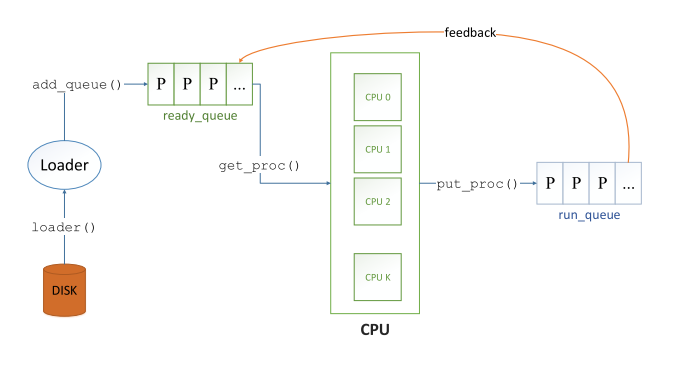
\includegraphics[width=1\textwidth]{scheduler.png}
    \caption{The operation of scheduler in the assignment}
    \label{fig:sched_figure}
\end{figure}

Our job in this part is to implement this algorithm by completing the following functions:

\begin{itemize}
    \item \mintinline{C}{enqueue()} and \mintinline{C}{dequeue()} (in \mintinline{C}{queue.c}): We have defined a struct \mintinline{C}{(queue_t)}\mintinline{C}{} for a priority queue at queue.h. Your task is to implement those functions to help put a new PCB to the queue and get a PCB with the highest priority out of the queue.
    \item \mintinline{C}{get_proc()} (in \mintinline{C}{sched.c}): gets PCB of a process waiting at ready queue. If the queue is empty at the time the function is called, you must move all PCBs of processes waiting at run queue back to ready queue before getting a process from ready queue.
\end{itemize}

\subsection{Memory Management}

The virtual memory engine uses Segmentation with Paging mechanism to manage the memory. By default, the size of virtual RAM is 1 MB so we must use 20 bit to represent the address of each of its byte. With the segmentation with paging mechanism, we use the first 5 bits for segment index, the next 5 bits for page index and the last 10 bits for offset. After that, you could implement the process of translating virtual address of a process to physical one by completing the following functions:
\begin{itemize}
    \item \mintinline{C}{get_page_table()} (in \mintinline{C}{mem.c}): Find the page table given a segment index of a process.
    \item \mintinline{C}{translate()} (in \mintinline{C}{mem.c}): uses get page \mintinline{C}{table()} function to translate a virtual address to physical address
\end{itemize}

Note that functions mentioned above are applied for processes which have already had segment table and page table for us to do our job. The main problem is how to construct those tables. Obviously, we cannot map the whole virtual address space of a process to RAM’s address space because RAM is shared by multiple processes and memory regions used by one process should not be used by other (ensure isolation). Therefore, we should start the process with empty segment table and keep updating it every time the process allocate or deallocate memory.

To simplify the implementation of memory allocation and deallocation, the OS maintains a special structure called \mintinline{C}{_mem_stat} which tracks the status of physical pages. Particularly, RAM is split into multiple pages according to Segmentation with Paging mechanism and the OS allocates memory to processes by pages. That is, if the process requires an amount of memory that less than the page size, it sill receives a whole new page. The responsibility of \mintinline{C}{_mem_stat} is to maintain the status (used/free) of those pages. Particularly, \mintinline{C}{_mem_stat} is a table in which each row is a struct defined as follows

\begin{mdframed}[leftline=true,rightline=true,backgroundcolor=white!10,nobreak=true]
  \begin{minted}[linenos,breaklines,breaksymbolleft=,obeytabs=true,tabsize=2]{R}
struct{
        uint32_t proc;
        uint32_t index;
        uint32_t next;
}
  \end{minted}
\end{mdframed}

where \mintinline{C}{proc} is the PID of the process which is currently use this page. If \mintinline{C}{proc} = 0, the page is free and the OS could allocated it to any process. Process may require a memory region whose size is much larger than the size of a single page. In this case, the OS must allocate multiple pages to this process. Since the process uses virtual address to access the content of RAM, we must let the virtual address of allocated pages contiguous but their physical addresses are not need to be. For example, support a process requires 2 pages and we have exactly 2 free pages in RAM but those page are not contiguous: the address of their first byte are \mintinline{C}{0x00000} and \mintinline{C}{0x01000}, respectively. In the virtual address space, we create two contiguous pages whose first byte are \mintinline{C}{0x00000} and \mintinline{C}{0x00020} (offset lasts 5 bits) and map page \mintinline{C}{0x00000} to physical page \mintinline{C}{0x00000}, page \mintinline{C}{0x00020} to physical page \mintinline{C}{0x01000}. Although process feels that the memory regions it has allocated is contiguous, they are actually not. Since we use this method for memory allocation, a row in \mintinline{C}{_mem_stat} has index field to know let us know its location in the list of allocated page. The next field is used to indicate the index in \mintinline{C}{_mem_stat} of next page in the list of allocated pages. If the page is the last page, this field is set to -1. In the previous example, the page \mintinline{C}{0x00000} has index = 0 and that of the page \mintinline{C}{0x01000} would be 1 while the value of their next are \mintinline{C}{0x80} and -1 respectively. This below figure shows how we allocate new memory regions and create new entry in the segment and page tables inside a process. Particularly, for each new page we allocated, we must add new entry to page tables according to this page’s segment number and page number.

\begin{figure}[H]
    \centering
    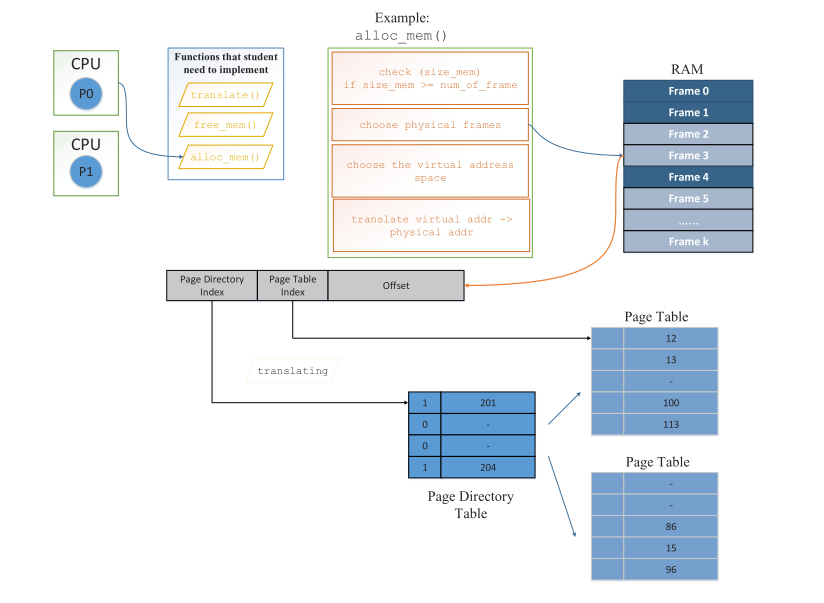
\includegraphics[width=1\textwidth]{mem_map.png}
    \caption{The operation related to virtual memory in the assignment}
    \label{fig:mem_manange_figure}
\end{figure}

Our main task is to implement functions \mintinline{C}{alloc_mem()} and \mintinline{C}{free_mem()} both are in \mintinline{C}{mem.c} based on the algorithm described above. 
\subsection{Put It All Together}

Finally, we combine scheduler and Virtual Memory Engine to form a complete OS. Figure 4 shows the complete organization of the OS. The last task to do is synchronization. Since the OS runs on multiple processors, it is possible that share resources could be concurrently accessed by more than one process at a time. Your job in this section is to find share resource and use lock mechanism to protect them.

\begin{figure}[H]
    \centering
    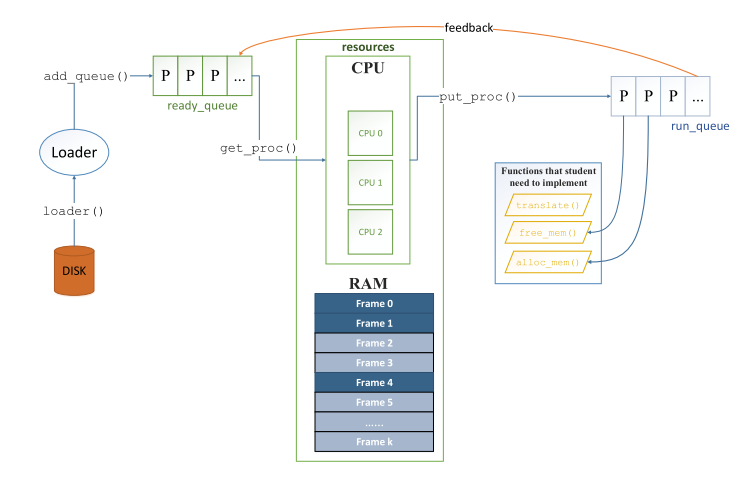
\includegraphics[width=1\textwidth]{os.png}
    \caption{The model of Assignment 2}
    \label{fig:os_figure}
\end{figure}

%TO DO%
\newpage
%%%%%%%%%%%%%%%%%%%%%%%%%%%%%%%%%

\section{Code Implementation}
%Job: implement code with guidance on how to do it%
\subsection{Scheduler}

\subsubsection{Priority Feedback Queue}

Before we can jump into code implementation, we must first understand the requirements intention when using Priority Feedback Queue:

\begin{itemize}
    \item The Priority Feedback Queue (PFQ) takes after some designing concept from the Multilevel Feedback Queue, i.e. using more than one queue to schedule process. 
    \item Within PFQ, the process with highest priority in queue will be executed first, if there are multiple processes with same priority, first process to be in the queue will be executed first (same as FCFS).
    \item The time slot— based on the Round Robins with Quantum time — is used to schedule the process.
\end{itemize}

A reason why PFQ has many advantages is because of its mechanism of prioritism, in which each defined process with higher priorities will be ran before others, solving starvation problems, ensuring all processes are executed.

The algorith also uses a time slot like Round-Robin algorith with a quantum time for each process, thus allowing tuning the quantum time to minimize average response and turnaround time.

Therefore, PFQ is a strict algorithm requiring the usage of 3 well-defined functions:
\begin{itemize}
    \item \mintinline{C}{enqueue() in queue.c}: adds a new process and sort the queue so higher priorities will be put first.
    \item \mintinline{C}{dequeue() in queue.c}: takes a process from the queue and update the queue.
    \item \mintinline{C}{get_proc() in sched.c}: dequeue a process from \mintinline{C}{ready_queue} to be put to \mintinline{C}{run_queue}.
\end{itemize}
\newpage
\subsubsection{queue.c}
\begin{itemize}
    \item \mintinline{C}{enqueue()}: When adding a new process in, there are 2 things to be noted: if the queue is empty or if the queue is full. Unlike dynamically allocated structure, the queue we have here is an array structure so any side conditions needs to be dealt with, which here in the code has been described thoroughly. 
    Note that we also use
\end{itemize}
\begin{mdframed}[leftline=true,rightline=true,backgroundcolor=blue!10,nobreak=true]
  \begin{minted}[linenos=true,breaklines,breaksymbolleft=,obeytabs=true,tabsize=2]{C}
void enqueue(struct queue_t * q, struct pcb_t * proc) {
	//if queue is empty, automatically assign the process
	if (empty(q)) 
	{
		q->proc[0] = proc;
		q->size += 1;
		return;
	}
	//Hold when queue is full
	while (q->size >= MAX_QUEUE_SIZE);
	//Finding index to put process (PFQ with FIFO)
	q->size += 1;
	for (int index = q->size - 1; index > 0; index--)
	{
		/*Check if the priority of index i-1 is lower than index
		So that when that process is done, proc will be the next 
		process*/
		if (q->proc[index-1]->priority <= proc->priority)
		{
			q->proc[index] = proc;
			break;
		}
		//Else shift right
		else
			q->proc[index] = q->proc[index-1];
		//When every process is shifted right, proc[0] = proc
		if (index == 1)
			q->proc[0] = proc;
	}
}
  \end{minted}
\end{mdframed}

\begin{itemize}
    \item \mintinline{C}{dequeue()}: When the hard work in \mintinline{C}{dequeue()} has been dealt with, the work in dequeue() is pretty simple, taking the head of the queue and update new head as well as moving all process indexes to the right (for space for new processes
\end{itemize}
\begin{mdframed}[leftline=true,rightline=true,backgroundcolor=blue!10,nobreak=true]
  \begin{minted}[linenos=true,breaklines,breaksymbolleft=,obeytabs=true,tabsize=2]{C}
struct pcb_t * dequeue(struct queue_t * q) {
	/* TODO: return a pcb whose prioprity is the highest
	 * in the queue [q] and remember to remove it from q
	 * */
	if (empty(q)) return NULL;
	struct pcb_t *result = q->proc[0];
	//Shifting processes to the left
	for (int i = 0; i < q->size - 1; i++)
	{
		q->proc[i] = q->proc[i+1];
	}
	q->size -= 1;
	return result;
}
  \end{minted}
\end{mdframed}
%TO DO%

\subsubsection{sched.c}

And finally, \mintinline{C}{get_proc()} moves a process from \mintinline{C}{ready_queue} to \mintinline{C}{run_queue}.
\begin{mdframed}[leftline=true,rightline=true,backgroundcolor=blue!10,nobreak=true]
  \begin{minted}[linenos=true,breaklines,breaksymbolleft=,obeytabs=true,tabsize=2]{C}
struct pcb_t * get_proc(void) {
	struct pcb_t * proc = NULL;
	/*TODO: get a process from [ready_queue]. If ready queue
	 * is empty, push all processes in [run_queue] back to
	 * [ready_queue] and return the highest priority one.
	 * Remember to use lock to protect the queue.
	 * */
	pthread_mutex_lock(&queue_lock);
	if (empty(&ready_queue)) {
		while (!empty(&run_queue)) {
			enqueue(&ready_queue, dequeue(&run_queue));
		}
	}
	if (empty(&ready_queue)==0) {
		proc = dequeue(&ready_queue);
	}
	pthread_mutex_unlock(&queue_lock);
	return proc;
}
  \end{minted}
\end{mdframed}

\subsection{Memory Management}
\subsubsection{Segmentation with Paging}
Segmentation with paging is a combination of both Segmentation and Paging techniques, where the main memory is divided into many segments with varying sizes and each segment houses a page table that further maps to many pages corresponding to frames in physical storage.

Upon a translation request is received, the Memory Management Unit will infer the position of the requested page from the virtual address by extracting the relevant bits, treating them as the indices to look for in the segment table and subsequently,the page table in said segment.

In the assignment, we will be modifying \mintinline{C}{mem.c} by completing \mintinline{C}{alloc_mem()} and \mintinline{C}{free_mem()} which are constructed by Segmentation in Paging. And also \mintinline{C}{translate()} to convert a virtual address to a the correlated physical address.

\subsubsection{\mintinline{C}{translate()}}
\begin{mdframed}[leftline=false,rightline=false,backgroundcolor=blue!10,nobreak=false]
  \begin{minted}[linenos=false,breaklines,breaksymbolleft=,obeytabs=true,tabsize=2]{text}
  static int translate(
		addr_t virtual_addr, 	// Given virtual address
		addr_t * physical_addr, // Physical address to be returned
		struct pcb_t * proc) {  // Process uses given virtual address

	/* Offset of the virtual address */
	addr_t offset = get_offset(virtual_addr);
	/* The first layer index */
	addr_t first_lv = get_first_lv(virtual_addr);
	/* The second layer index */
	addr_t second_lv = get_second_lv(virtual_addr);
	
	/* Search in the first level */
	struct page_table_t * page_table = NULL;
	page_table = get_page_table(first_lv, proc->seg_table);
	if (page_table == NULL) {
		return 0;
	}

	int i;
	for (i = 0; i < page_table->size; i++) {
		if (page_table->table[i].v_index == second_lv) {
			addr_t physical_index = page_table->table[i].p_index;
			*physical_addr = (physical_index << OFFSET_LEN) | (offset);
            return 1;
		}
	}
	return 0;	
}
  \end{minted}
\end{mdframed}

\subsubsection{\mintinline{C}{free_mem()}}

\begin{mdframed}[leftline=false,rightline=false,backgroundcolor=blue!10,nobreak=false]
  \begin{minted}[linenos=false,breaklines,breaksymbolleft=,obeytabs=true,tabsize=2]{text}
int free_mem(addr_t address, struct pcb_t *proc)
{
    pthread_mutex_lock(&mem_lock);
    addr_t p_address = 0;       // Physical address to free in memory
    addr_t v_address = address; // Virtual address to free in process
    // * Valid virtual address or not
    if (!translate(v_address, &p_address, proc))
	{
		pthread_mutex_unlock(&mem_lock);
		return 1;
	}
    // * Clear physical page in memmory
    addr_t p_segment_page_index = p_address >> OFFSET_LEN;
    int num_pages = 0; // Number of pages in list
    for (int i = p_segment_page_index; i != -1; i = _mem_stat[i].next)
    {
        _mem_stat[i].proc = 0;
        num_pages++;
    }
    // * Clear virtual page in process
    for (int i = 0; i < num_pages; i++)
    {
        addr_t v_addr = v_address + i * PAGE_SIZE;
        addr_t v_segment = get_first_lv(v_addr);
        addr_t v_page = get_second_lv(v_addr);
        struct page_table_t *page_table = get_page_table(v_segment, proc->seg_table);
        int j;
        for ( j = 0; j < page_table->size; j++)
        {
            if (page_table->table[j].v_index == v_page)
            {
                int last_index_page_table = page_table->size - 1;
                page_table->table[j] = page_table->table[last_index_page_table];
                break;
            }
        }
        if (page_table->size == 0)
        {
            struct seg_table_t *seg_table = proc->seg_table; // Get page table from proc
            if (seg_table != NULL){
            for (int z = 0; z < seg_table->size; z++)
            {
                if (seg_table->table[z].v_index == v_segment){
                int last_index_page_table = seg_table->size - 1;
                seg_table->table[z] = seg_table->table[last_index_page_table];
                seg_table->table[last_index_page_table].v_index = 0;
                free(seg_table->table[last_index_page_table].pages);
                seg_table->size--;
            }
        }
    }
}
}
  // * Update break pointer
    if (v_address + num_pages * PAGE_SIZE == proc->bp)
    {
        while (proc->bp >= PAGE_SIZE)
        {
            addr_t last_addr = proc->bp - PAGE_SIZE;
            addr_t last_segment = get_first_lv(last_addr);
            addr_t last_page = get_second_lv(last_addr);
            struct page_table_t *page_table = get_page_table(last_segment, proc->seg_table);
            if (page_table == NULL)
                break;
            while (last_page >= 0)
            {
                int i;
                for (i = 0; i < page_table->size; i++)
                {
                    if (page_table->table[i].v_index == last_page)
                    {
                        proc->bp -= PAGE_SIZE;
                        last_page--;
                        break;
                    }
                }
                if (i == page_table->size)
                    break;
            }
            if (last_page >= 0)
                break;
        }
    }
    pthread_mutex_unlock(&mem_lock);
    return 0;
}
  \end{minted}
\end{mdframed}

\subsubsection{\mintinline{C}{alloc_mem()}}

\begin{mdframed}[leftline=false,rightline=false,backgroundcolor=blue!10,nobreak=false]
  \begin{minted}[linenos=false,breaklines,breaksymbolleft=,obeytabs=true,tabsize=2]{text}
addr_t alloc_mem(uint32_t size, struct pcb_t *proc)
{
    pthread_mutex_lock(&mem_lock);
    addr_t ret_mem = 0;
    /* TODO: Allocate [size] byte in the memory for the
	 * process [proc] and save the address of the first
	 * byte in the allocated memory region to [ret_mem].
	 * */

    uint32_t num_pages = (size % PAGE_SIZE) ? size / PAGE_SIZE + 1 : size / PAGE_SIZE; // Number of pages we will use for this proc

    int mem_avail = 1; // We could allocate new memory region or not?

    int free_pages = 0;
    for (int i = 0; i < NUM_PAGES; i++)
    {
        if (_mem_stat[i].proc == 0)
            free_pages = free_pages + 1;
        if (free_pages == NUM_PAGES)
            break;
    }

    if (free_pages < num_pages)
        mem_avail = 0;

    if (proc->bp + num_pages * PAGE_SIZE >= RAM_SIZE)
        mem_avail = 0;

    /* First we must check if the amount of free memory in
	 * virtual address space and physical address space is
	 * large enough to represent the amount of required 
	 * memory. If so, set 1 to [mem_avail].
	 * Hint: check [proc] bit in each page of _mem_stat
	 * to know whether this page has been used by a process.
	 * For virtual memory space, check bp (break pointer).
	 * */

    if (mem_avail)
    {
        /* We could allocate new memory region to the process */
        ret_mem = proc->bp;
        proc->bp += num_pages * PAGE_SIZE;
        /* Update status of physical pages which will be allocated
		 * to [proc] in _mem_stat. Tasks to do:
		 * 	- Update [proc], [index], and [next] field
		 * 	- Add entries to segment table page tables of [proc]
		 * 	  to ensure accesses to allocated memory slot is
		 * 	  valid. */

        int allocate_pages = 0;             // count allocated pages
        int last_allocated_page_index = -1; // use for update field [next] of last allocated page
        for (int i = 0; i < NUM_PAGES; i++)
        {
            if (_mem_stat[i].proc != 0)
                continue;

            // * Update proc and index for this page
            _mem_stat[i].proc = proc->pid;
            _mem_stat[i].index = allocate_pages;

            // * Update last page
            if (last_allocated_page_index > -1)
            {
                _mem_stat[last_allocated_page_index].next = i;
            }
            last_allocated_page_index = i;

            // * Virtual page table
            addr_t v_address = ret_mem + allocate_pages * PAGE_SIZE;
            addr_t v_segment = get_first_lv(v_address);

            struct page_table_t *v_page_table = get_page_table(v_segment, proc->seg_table);
            if (v_page_table == NULL)
            {
                int idx = proc->seg_table->size;
                proc->seg_table->table[idx].v_index = v_segment;
                v_page_table = proc->seg_table->table[idx].pages = (struct page_table_t *)malloc(sizeof(struct page_table_t));
                proc->seg_table->size++;
            }
            int idx = v_page_table->size++;
            v_page_table->table[idx].v_index = get_second_lv(v_address);
            v_page_table->table[idx].p_index = i;
            allocate_pages = allocate_pages + 1;

            if (allocate_pages == num_pages)
            {
                _mem_stat[i].next = -1; // last page in list
                break;
            }
        }
    }
    pthread_mutex_unlock(&mem_lock);
    return ret_mem;
}
  \end{minted}
\end{mdframed}
%TO DO%

%%%%%%%%%%%%%%%%%%%%%%%%%%%%%%%%%

\section{Observation And Conclusion}
%Job: complete section 3.2 of the assignment
%TO DO%

\subsection{Scheduler}

Here, we will use \mintinline{C}{input/sched_0} and \mintinline{C}{input/sched_1} as our input file, and the output file will be compared to \mintinline{C}{output/sched_0} and \mintinline{C}{output/sched_1}.
\textit{NOTE: all files can be found in the folders in ZIP files.}

\begin{itemize}
    \item \mintinline{C}{sched_0}
\end{itemize}

\begin{table}[H]
  \centering
  \begin{tabular}{cccc}
    \toprule
    Process & Arrival time & Burst Time & Priority \\
    \midrule
    s0      & 0            & 15         & 12       \\
    s1      & 4            & 7          & 20       \\
    \bottomrule
  \end{tabular}
\end{table}

With Gantt Diagram:

\begin{figure}[H]
  \centering
  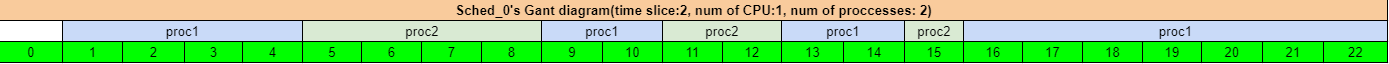
\includegraphics[width=1\textwidth]{sche0_gantt.png}
  \caption{Gantt diagram of \mintinline{C}{sched_0}}
\end{figure}

Output from the program:

\begin{mdframed}[leftline=false,rightline=false,backgroundcolor=grey!10,nobreak=false]
  \begin{minted}[linenos=false,breaklines,breaksymbolleft=,obeytabs=true,tabsize=2]{text}
  ------ SCHEDULING TEST 0 -------------------------------------------
./os sched_0
Time slot   0
        Loaded a process at input/proc/s0, PID: 1
Time slot   1
        CPU 0: Dispatched process  1
Time slot   2
Time slot   3
        CPU 0: Put process  1 to run queue
        CPU 0: Dispatched process  1
        Loaded a process at input/proc/s1, PID: 2
Time slot   4
Time slot   5
        CPU 0: Put process  1 to run queue
        CPU 0: Dispatched process  2
Time slot   6
Time slot   7
        CPU 0: Put process  2 to run queue
        CPU 0: Dispatched process  1
Time slot   8
Time slot   9
        CPU 0: Put process  1 to run queue
        CPU 0: Dispatched process  2
Time slot  10
Time slot  11
        CPU 0: Put process  2 to run queue
        CPU 0: Dispatched process  1
Time slot  12
Time slot  13
        CPU 0: Put process  1 to run queue
        CPU 0: Dispatched process  2
Time slot  14
Time slot  15
        CPU 0: Put process  2 to run queue
        CPU 0: Dispatched process  1
Time slot  16
Time slot  17
        CPU 0: Put process  1 to run queue
        CPU 0: Dispatched process  2
Time slot  18
        CPU 0: Processed  2 has finished
        CPU 0: Dispatched process  1
Time slot  19
Time slot  20
        CPU 0: Put process  1 to run queue
        CPU 0: Dispatched process  1
Time slot  21
Time slot  22
        CPU 0: Put process  1 to run queue
        CPU 0: Dispatched process  1
Time slot  23
        CPU 0: Processed  1 has finished
        CPU 0 stopped

MEMORY CONTENT: 
NOTE: Read file output/sched_0 to verify your result
  \end{minted}
\end{mdframed}

\begin{itemize}
    \item \mintinline{C}{sched_1}
\end{itemize}

\begin{table}[H]
  \centering
  \begin{tabular}{cccc}
    \toprule
    Process & Arrival time & Burst Time & Priority \\
    \midrule
    s0      & 0            & 15         & 12       \\
    s1      & 4            & 7          & 20       \\
    s2      & 6            & 12         & 20       \\
    s3      & 7            & 11         & 7        \\
    \bottomrule
  \end{tabular}
\end{table}

With Gantt Diagram:

\begin{figure}[H]
  \centering
  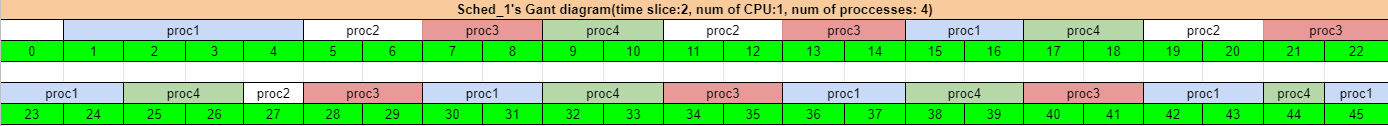
\includegraphics[width=1\textwidth]{sche1_gantt.png}
  \caption{Gantt diagram of \mintinline{C}{sched_1}}
\end{figure}

Output from the program:
\begin{mdframed}[leftline=false,rightline=false,backgroundcolor=grey!10,nobreak=false]
  \begin{minted}[linenos=false,breaklines,breaksymbolleft=,obeytabs=true,tabsize=2]{text}
------ SCHEDULING TEST 1 ---------------------
./os sched_1
Time slot   0
        Loaded a process at input/proc/s0, PID: 1
Time slot   1
        CPU 0: Dispatched process  1
Time slot   2
Time slot   3
        CPU 0: Put process  1 to run queue
        CPU 0: Dispatched process  1
        Loaded a process at input/proc/s1, PID: 2
Time slot   4
Time slot   5
        CPU 0: Put process  1 to run queue
        CPU 0: Dispatched process  2
        Loaded a process at input/proc/s2, PID: 3
Time slot   6
Time slot   7
        CPU 0: Put process  2 to run queue
        CPU 0: Dispatched process  3
        Loaded a process at input/proc/s3, PID: 4
Time slot   8
Time slot   9
        CPU 0: Put process  3 to run queue
        CPU 0: Dispatched process  4
Time slot  10
Time slot  11
        CPU 0: Put process  4 to run queue
        CPU 0: Dispatched process  4
Time slot  12
Time slot  13
        CPU 0: Put process  4 to run queue
        CPU 0: Dispatched process  1
Time slot  14
Time slot  15
        CPU 0: Put process  1 to run queue
        CPU 0: Dispatched process  2
Time slot  16
Time slot  17
        CPU 0: Put process  2 to run queue
        CPU 0: Dispatched process  3
Time slot  18
Time slot  19
        CPU 0: Put process  3 to run queue
        CPU 0: Dispatched process  4
Time slot  20
Time slot  21
        CPU 0: Put process  4 to run queue
        CPU 0: Dispatched process  1
Time slot  22
Time slot  23
        CPU 0: Put process  1 to run queue
        CPU 0: Dispatched process  2
Time slot  24
Time slot  25
        CPU 0: Put process  2 to run queue
        CPU 0: Dispatched process  3
Time slot  26
Time slot  27
        CPU 0: Put process  3 to run queue
        CPU 0: Dispatched process  4
Time slot  28
Time slot  29
        CPU 0: Put process  4 to run queue
        CPU 0: Dispatched process  1
Time slot  30
Time slot  31
        CPU 0: Put process  1 to run queue
        CPU 0: Dispatched process  2
Time slot  32
        CPU 0: Processed  2 has finished
        CPU 0: Dispatched process  3
Time slot  33
Time slot  34
        CPU 0: Put process  3 to run queue
        CPU 0: Dispatched process  4
Time slot  35
Time slot  36
        CPU 0: Put process  4 to run queue
        CPU 0: Dispatched process  1
Time slot  37
Time slot  38
        CPU 0: Put process  1 to run queue
        CPU 0: Dispatched process  3
Time slot  39
Time slot  40
        CPU 0: Put process  3 to run queue
        CPU 0: Dispatched process  4
Time slot  41
        CPU 0: Processed  4 has finished
        CPU 0: Dispatched process  1
Time slot  42
Time slot  43
        CPU 0: Put process  1 to run queue
        CPU 0: Dispatched process  3
Time slot  44
Time slot  45
        CPU 0: Processed  3 has finished
        CPU 0: Dispatched process  1
Time slot  46
        CPU 0: Processed  1 has finished
        CPU 0 stopped
MEMORY CONTENT:
  \end{minted}
\end{mdframed}

\subsection{Memory Management}
Here, we will use \mintinline{C}{input/proc/m0} and \mintinline{C}{input/proc/m1} as our input file, and the output will be compared to \mintinline{C}{output/mem_0} and \mintinline{C}{output/mem_1}.
\textit{NOTE: all files can be found in the folders in ZIP files.}
\begin{mdframed}[leftline=false,rightline=false,backgroundcolor=grey!10,nobreak=false]
  \begin{minted}[linenos=false,breaklines,breaksymbolleft=,obeytabs=true,tabsize=2]{text}
  ------ MEMORY MANAGEMENT TEST 0 ------------------------------------
./mem input/proc/m0
000: 00000-003ff - PID: 01 (idx 000, nxt: 001)
        003e8: 15
001: 00400-007ff - PID: 01 (idx 001, nxt: -01)
002: 00800-00bff - PID: 01 (idx 000, nxt: 003)
003: 00c00-00fff - PID: 01 (idx 001, nxt: 004)
004: 01000-013ff - PID: 01 (idx 002, nxt: 005)
005: 01400-017ff - PID: 01 (idx 003, nxt: 006)
006: 01800-01bff - PID: 01 (idx 004, nxt: -01)
014: 03800-03bff - PID: 01 (idx 000, nxt: 015)
        03814: 66
015: 03c00-03fff - PID: 01 (idx 001, nxt: -01)
  \end{minted}
\end{mdframed}

\begin{mdframed}[leftline=false,rightline=false,backgroundcolor=grey!10,nobreak=false]
  \begin{minted}[linenos=false,breaklines,breaksymbolleft=,obeytabs=true,tabsize=2]{text}
  ------ MEMORY MANAGEMENT TEST 1 ------------------------------------
./mem input/proc/m1
  \end{minted}
\end{mdframed}
\subsection{Put It All Together}
Here, we will use \mintinline{C}{input/os_0} and \mintinline{C}{input/os_1} as our input file, and the output will be compared to \mintinline{C}{output/os_0} and \mintinline{C}{output/os_1}.
\textit{NOTE: all files can be found in the folders in ZIP files.}
\begin{mdframed}[leftline=false,rightline=false,backgroundcolor=grey!10,nobreak=false]
  \begin{minted}[linenos=false,breaklines,breaksymbolleft=,obeytabs=true,tabsize=2]{text}
  ----- OS TEST 0 ----------------------------------------------------
./os os_0
Time slot   0
        Loaded a process at input/proc/p0, PID: 1
        CPU 1: Dispatched process  1
Time slot   1
        Loaded a process at input/proc/p1, PID: 2
Time slot   2
        CPU 0: Dispatched process  2
        Loaded a process at input/proc/p1, PID: 3
Time slot   3
        Loaded a process at input/proc/p1, PID: 4
Time slot   4
Time slot   5
        CPU 1: Put process  1 to run queue
        CPU 1: Dispatched process  3
Time slot   6
Time slot   7
Time slot   8
        CPU 0: Put process  2 to run queue
        CPU 0: Dispatched process  4
Time slot   9
Time slot  10
Time slot  11
        CPU 1: Put process  3 to run queue
Time slot  12
        CPU 1: Dispatched process  1
Time slot  13
Time slot  14
        CPU 0: Put process  4 to run queue
        CPU 0: Dispatched process  2
Time slot  15
Time slot  16
        CPU 1: Processed  1 has finished
        CPU 1: Dispatched process  3
Time slot  17
Time slot  18
        CPU 0: Processed  2 has finished
        CPU 0: Dispatched process  4
Time slot  19
        CPU 1: Processed  3 has finished
        CPU 1 stopped
Time slot  20
Time slot  21
Time slot  22
        CPU 0: Processed  4 has finished
        CPU 0 stopped

MEMORY CONTENT: 
000: 00000-003ff - PID: 02 (idx 000, nxt: 001)
001: 00400-007ff - PID: 02 (idx 001, nxt: 007)
002: 00800-00bff - PID: 02 (idx 000, nxt: 003)
003: 00c00-00fff - PID: 02 (idx 001, nxt: 004)
004: 01000-013ff - PID: 02 (idx 002, nxt: 005)
005: 01400-017ff - PID: 02 (idx 003, nxt: -01)
006: 01800-01bff - PID: 03 (idx 000, nxt: 033)
007: 01c00-01fff - PID: 02 (idx 002, nxt: 008)
        01de7: 0a
008: 02000-023ff - PID: 02 (idx 003, nxt: 009)
009: 02400-027ff - PID: 02 (idx 004, nxt: -01)
010: 02800-02bff - PID: 01 (idx 000, nxt: -01)
        02814: 64
011: 02c00-02fff - PID: 02 (idx 000, nxt: 012)
012: 03000-033ff - PID: 02 (idx 001, nxt: 013)
013: 03400-037ff - PID: 02 (idx 002, nxt: 014)
014: 03800-03bff - PID: 02 (idx 003, nxt: -01)
015: 03c00-03fff - PID: 03 (idx 000, nxt: 016)
016: 04000-043ff - PID: 03 (idx 001, nxt: 017)
017: 04400-047ff - PID: 03 (idx 002, nxt: 018)
        045e7: 0a
018: 04800-04bff - PID: 03 (idx 003, nxt: 019)
019: 04c00-04fff - PID: 03 (idx 004, nxt: -01)
020: 05000-053ff - PID: 04 (idx 000, nxt: 021)
021: 05400-057ff - PID: 04 (idx 001, nxt: 022)
022: 05800-05bff - PID: 04 (idx 002, nxt: 023)
        059e7: 0a
023: 05c00-05fff - PID: 04 (idx 003, nxt: 024)
024: 06000-063ff - PID: 04 (idx 004, nxt: -01)
025: 06400-067ff - PID: 03 (idx 000, nxt: 026)
026: 06800-06bff - PID: 03 (idx 001, nxt: 027)
027: 06c00-06fff - PID: 03 (idx 002, nxt: 028)
028: 07000-073ff - PID: 03 (idx 003, nxt: -01)
029: 07400-077ff - PID: 04 (idx 000, nxt: 030)
030: 07800-07bff - PID: 04 (idx 001, nxt: 031)
031: 07c00-07fff - PID: 04 (idx 002, nxt: 032)
032: 08000-083ff - PID: 04 (idx 003, nxt: -01)
033: 08400-087ff - PID: 03 (idx 001, nxt: 034)
034: 08800-08bff - PID: 03 (idx 002, nxt: 035)
035: 08c00-08fff - PID: 03 (idx 003, nxt: -01)
036: 09000-093ff - PID: 04 (idx 000, nxt: 037)
037: 09400-097ff - PID: 04 (idx 001, nxt: 038)
038: 09800-09bff - PID: 04 (idx 002, nxt: 039)
039: 09c00-09fff - PID: 04 (idx 003, nxt: -01)
  \end{minted}
\end{mdframed}


\begin{mdframed}[leftline=false,rightline=false,backgroundcolor=grey!10,nobreak=false]
  \begin{minted}[linenos=false,breaklines,breaksymbolleft=,obeytabs=true,tabsize=2]{text}
  ----- OS TEST 1 ----------------------------------------------------
./os os_1
Time slot   0
        Loaded a process at input/proc/p0, PID: 1
Time slot   1
        CPU 0: Dispatched process  1
        Loaded a process at input/proc/s3, PID: 2
Time slot   2
        CPU 3: Dispatched process  2
Time slot   3
        CPU 0: Put process  1 to run queue
        CPU 0: Dispatched process  1
        Loaded a process at input/proc/m1, PID: 3
        CPU 2: Dispatched process  3
Time slot   4
        CPU 3: Put process  2 to run queue
        CPU 3: Dispatched process  2
Time slot   5
        CPU 0: Put process  1 to run queue
        CPU 0: Dispatched process  1
        Loaded a process at input/proc/s2, PID: 4
        CPU 2: Put process  3 to run queue
        CPU 2: Dispatched process  3
Time slot   6
        CPU 1: Dispatched process  4
        CPU 3: Put process  2 to run queue
        CPU 3: Dispatched process  2
Time slot   7
        Loaded a process at input/proc/m0, PID: 5
        CPU 0: Put process  1 to run queue
        CPU 0: Dispatched process  5
        CPU 2: Put process  3 to run queue
        CPU 1: Put process  4 to run queue
        CPU 1: Dispatched process  1
        CPU 2: Dispatched process  4
Time slot   8
        Loaded a process at input/proc/p1, PID: 6
Time slot   9
        CPU 0: Put process  5 to run queue
        CPU 0: Dispatched process  6
        CPU 3: Put process  2 to run queue
        CPU 3: Dispatched process  3
        CPU 2: Put process  4 to run queue
        CPU 2: Dispatched process  5
Time slot  10
        CPU 1: Put process  1 to run queue
        CPU 1: Dispatched process  2
        Loaded a process at input/proc/s0, PID: 7
Time slot  11
        CPU 3: Put process  3 to run queue
        CPU 3: Dispatched process  7
        CPU 0: Put process  6 to run queue
        CPU 0: Dispatched process  1
        CPU 2: Put process  5 to run queue
        CPU 2: Dispatched process  3
        CPU 1: Put process  2 to run queue
        CPU 1: Dispatched process  6
Time slot  12
        CPU 3: Put process  7 to run queue
        CPU 3: Dispatched process  4
Time slot  13
        CPU 0: Processed  1 has finished
        CPU 0: Dispatched process  5
        CPU 2: Processed  3 has finished
Time slot  14
        CPU 2: Dispatched process  2
        CPU 1: Put process  6 to run queue
        CPU 1: Dispatched process  7
        CPU 3: Put process  4 to run queue
        CPU 3: Dispatched process  6
Time slot  15
        CPU 0: Put process  5 to run queue
        CPU 0: Dispatched process  4
        Loaded a process at input/proc/s1, PID: 8
        CPU 2: Put process  2 to run queue
        CPU 2: Dispatched process  8
Time slot  16
        CPU 1: Put process  7 to run queue
        CPU 1: Dispatched process  5
        CPU 3: Put process  6 to run queue
        CPU 3: Dispatched process  2
        CPU 1: Processed  5 has finished
        CPU 1: Dispatched process  7
        CPU 0: Put process  4 to run queue
        CPU 0: Dispatched process  6
Time slot  17
        CPU 3: Processed  2 has finished
Time slot  18
        CPU 3: Dispatched process  4
        CPU 2: Put process  8 to run queue
        CPU 2: Dispatched process  8
        CPU 1: Put process  7 to run queue
        CPU 1: Dispatched process  7
        CPU 0: Put process  6 to run queue
        CPU 0: Dispatched process  6
Time slot  19
        CPU 3: Put process  4 to run queue
Time slot  20
        CPU 3: Dispatched process  4
        CPU 2: Put process  8 to run queue
        CPU 2: Dispatched process  8
Time slot  21
        CPU 1: Put process  7 to run queue
        CPU 1: Dispatched process  7
        CPU 0: Processed  6 has finished
        CPU 0 stopped
        CPU 3: Processed  4 has finished
        CPU 3 stopped
        CPU 2: Put process  8 to run queue
        CPU 2: Dispatched process  8
Time slot  22
        CPU 2: Processed  8 has finished
        CPU 1: Put process  7 to run queue
        CPU 1: Dispatched process  7
        CPU 2 stopped
Time slot  23
Time slot  24
Time slot  25
        CPU 1: Put process  7 to run queue
        CPU 1: Dispatched process  7
Time slot  26
Time slot  27
        CPU 1: Put process  7 to run queue
        CPU 1: Dispatched process  7
Time slot  28
        CPU 1: Processed  7 has finished
        CPU 1 stopped

MEMORY CONTENT: 
000: 00000-003ff - PID: 06 (idx 000, nxt: 001)
001: 00400-007ff - PID: 06 (idx 001, nxt: 031)
002: 00800-00bff - PID: 05 (idx 000, nxt: 003)
003: 00c00-00fff - PID: 05 (idx 001, nxt: 004)
004: 01000-013ff - PID: 05 (idx 002, nxt: 005)
005: 01400-017ff - PID: 05 (idx 003, nxt: 006)
006: 01800-01bff - PID: 05 (idx 004, nxt: -01)
007: 01c00-01fff - PID: 05 (idx 000, nxt: 008)
        01fe8: 15
008: 02000-023ff - PID: 05 (idx 001, nxt: -01)
009: 02400-027ff - PID: 06 (idx 000, nxt: 010)
010: 02800-02bff - PID: 06 (idx 001, nxt: 011)
011: 02c00-02fff - PID: 06 (idx 002, nxt: 012)
012: 03000-033ff - PID: 06 (idx 003, nxt: -01)
013: 03400-037ff - PID: 06 (idx 000, nxt: 014)
014: 03800-03bff - PID: 06 (idx 001, nxt: 015)
015: 03c00-03fff - PID: 06 (idx 002, nxt: 016)
016: 04000-043ff - PID: 06 (idx 003, nxt: -01)
021: 05400-057ff - PID: 01 (idx 000, nxt: -01)
        05414: 64
024: 06000-063ff - PID: 05 (idx 000, nxt: 025)
        06014: 66
025: 06400-067ff - PID: 05 (idx 001, nxt: -01)
031: 07c00-07fff - PID: 06 (idx 002, nxt: 032)
        07de7: 0a
032: 08000-083ff - PID: 06 (idx 003, nxt: 033)
033: 08400-087ff - PID: 06 (idx 004, nxt: -01)
  \end{minted}
\end{mdframed}
%%%%%%%%%%%%%%%%%%%%%%%%%%%%%%%%%
\end{document}